\documentclass{article}

\usepackage{titlesec}
\usepackage{longtable}
\usepackage{array} % for defining a new column type
\usepackage{varwidth} %for the varwidth minipage environment
\usepackage{color, colortbl}
\usepackage{caption}
\usepackage{subfigure}
\usepackage{filecontents}
\usepackage[section]{placeins}
\usepackage{float}
\usepackage{lscape}

\definecolor{Gray}{gray}{0.9}

\usepackage{pgf-umlsd}
\usepackage{pgf-umlcd}

\usepackage[latin1]{inputenc}
\usepackage{tikz}
\usetikzlibrary{shapes,arrows}

\newcommand{\sectionbreak}{\clearpage}

\begin{document}


\tikzstyle{decision} = [diamond, draw, fill=blue!20, 
    text width=4.5em, text badly centered, node distance=3cm, inner sep=0pt]
\tikzstyle{block} = [rectangle, draw, fill=blue!20, 
    text width=5em, text centered, rounded corners, minimum height=4em]
\tikzstyle{line} = [draw, -latex']
\tikzstyle{cloud} = [draw, ellipse,fill=red!20, node distance=3cm,
    minimum height=2em]

\newcolumntype{M}{>{\begin{varwidth}{4cm}}l<{\end{varwidth}}} %M is for Maximal column

\begin{titlepage}
	\Huge{Bitcode Assignment 2}
\end{titlepage}


\section{Design Patterns}
Using design patterns in software project is a good practice. It helps to make your software understandable, sustainable and expendable. We have chosen two design patterns and implemented them in our existing code, the observer pattern and the factory pattern.

\subsection{The Observer Design Pattern}
The observer pattern is implemented between the MouseActionHandler class (subject) and the DragAnimation class (observer). The MouseActionHandler listens for mouse input in a given window. A object of the DragAnimation class is created when a mouse drag is registered and updated when the position of the mouse pointer changes. 
\paragraph{} We have chosen this pattern on this location because it enables us to create more observers for the MouseActionHandler in the future. Therefore it will save time to implement new features that need the MouseActionHandler class.
 

\subsubsection{Observer Class Diagram}
\begin{figure}[H]
	\centering
	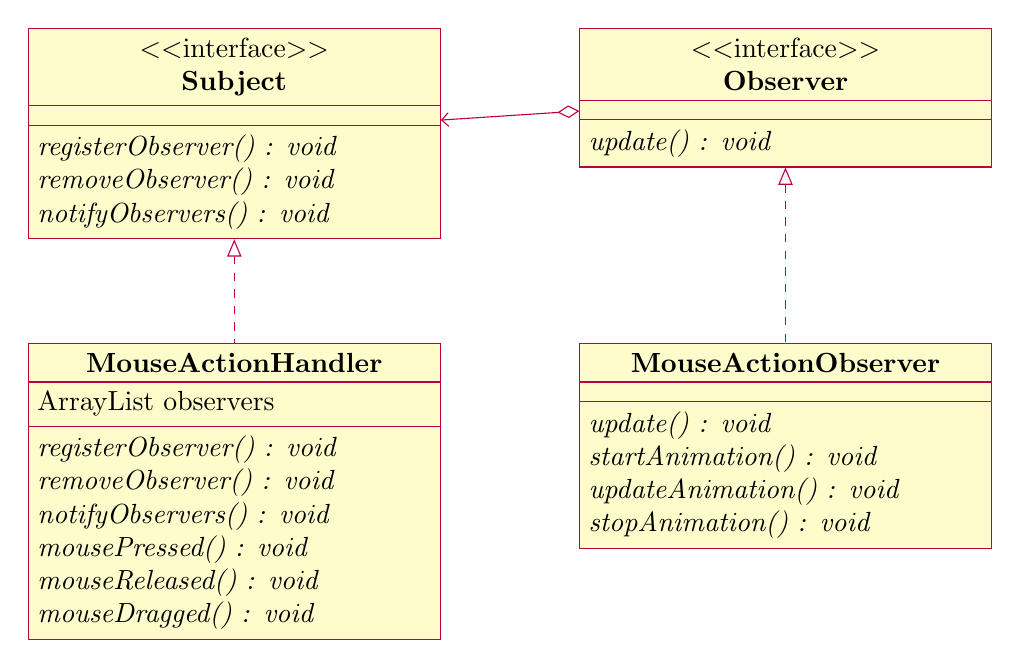
\begin{tikzpicture}
		\begin{interface}{Subject}{-3,0}
			\operation[0]{registerObserver() : void}
			\operation[0]{removeObserver() : void}
			\operation[0]{notifyObservers() : void}
		\end{interface}
		\begin{class}{MouseActionHandler}{-3,-4}
			\implement{Subject}
			\attribute{ArrayList observers}
			\operation[0]{registerObserver() : void}
			\operation[0]{removeObserver() : void}
			\operation[0]{notifyObservers() : void}
			\operation[0]{mousePressed() : void}
			\operation[0]{mouseReleased() : void}
			\operation[0]{mouseDragged() : void}
		\end{class}
		
		\begin{interface}{Observer}{4,0} 
			\operation[0]{update() : void}
		\end{interface}
		\begin{class}{MouseActionObserver}{4,-4}
			\implement{Observer}
			\operation[0]{update() : void}
			\operation[0]{startAnimation() : void}
			\operation[0]{updateAnimation() : void}
			\operation[0]{stopAnimation() : void}
		\end{class}
		
		\aggregation{Observer}{}{}{Subject}
		
	\end{tikzpicture}
\end{figure}

\newpage
\subsubsection{Observer Sequence Diagram}
\begin{figure}[H]
	\centering
	\begin{sequencediagram}
		\newinst[1]{C}{:DragAnimation}{}
		\newthread{A}{:MouseActionObserver}{}
		\newthread{B}{:MouseEventHandler}{}
		\begin{call}{A}{registerObserver()}{B}{}
		\end{call}
		\begin{sdblock}{Event}{mouse dragged}
			\begin{call}{B}{update()}{A}{}
				\begin{call}{A}{getMouseAction()}{B}{}
				\end{call}
				\begin{call}{A}{start()}{C}{}
				\end{call}
			\end{call}
		\end{sdblock}
	\end{sequencediagram}
\end{figure}

\subsection{The Factory Design Pattern}
The factory design patterns are implemented for the BoardFactory and the ItemFactory. On launch the board is created via the StandardBoardFactory which will construct a board using the StandardItemFactory.
\paragraph{} The reason that we have implemented a factory pattern for the Board class is that we can use this pattern in the future for creating different types of board. For instance creating boards with different sizes based on difficulty. 
\paragraph{} We have implemented the factory pattern for the Item class because that allows us to create different types of items in the board, such as special items that will remove all items from the board.

\subsubsection{Factory Class Diagram}
\begin{figure}[H]
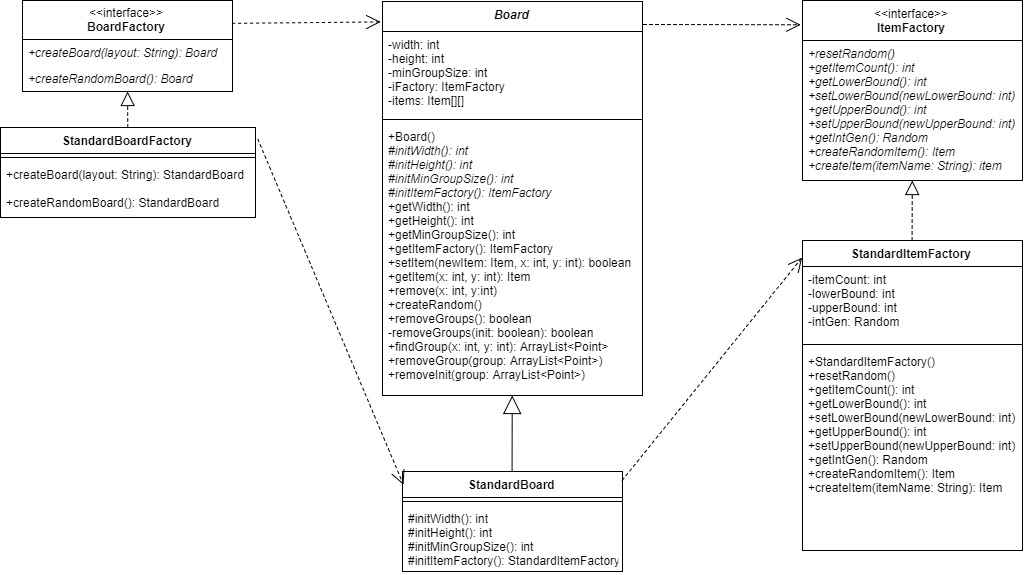
\includegraphics[scale=0.43]{Images/FactoriesClassDiagram.jpg}
\end{figure}

\subsubsection{Factory Sequence Diagram} 
\begin{figure}[H]
	\centering
	\begin{sequencediagram}
		\newthread{A}{:Game}{}
		\newinst[1]{B}{:StandardBoardFactory}{}
		\newinst[1]{C}{:StandardItemFactory}{}
		\begin{call}{A}{createBoard()}{B}{}
			\begin{call}{B}{Loop}{B}{}
				\begin{call}{B}{createItem()}{C}{}
				\end{call}
			\end{call}
		\end{call}
	\end{sequencediagram}
\end{figure}

\newpage
\section{Your wish is my command}
Our client wanted to have two new features implemented, which consist of a high score page and maximum amount of moves per level. For each each feature we have created new requirements and a software design.

\subsection{High Score Page} 
Having a High Score page, allows the player to keep track of his/her progress as the game is played. This is fun on its own but also allows the player to be competitive with other people playing the game, by comparing high scores. The high score page should be a top ten list of the highest scores in the game. When a player scores higher than the lowest of the top ten, then the player should be able to add their name to the list and bump the lowest, of the now eleven, of the list. The high score page should also have a save file, so that the progress is not lost when the player closes the game. Loading and saving should be done automatically.

\subsubsection{Requirements}
The requirement that are sorted using the MoSCoW model.

\paragraph{Must Have}
\begin{itemize}
\item At the end of the game, The player must be able to enter a name.

\item At the end of the game, The score of the player must be saved in a save file if the score is among the ten highest ranking in the save file.

\item At the end of the game, If the player is amongst the ten highest ranking in top ten high scores then allow the player to enter his name and add the score to the lists. Number 10, which has now become number 11 should be removed from the list and save file.

\item If no save file exists on the computer the game must create one.
\end{itemize}



\subsubsection{Software Design}
In order to implement the score board we have chosen to use the state design pattern. In the figure below is shown how the state pattern could be implemented.

\begin{figure}[H]
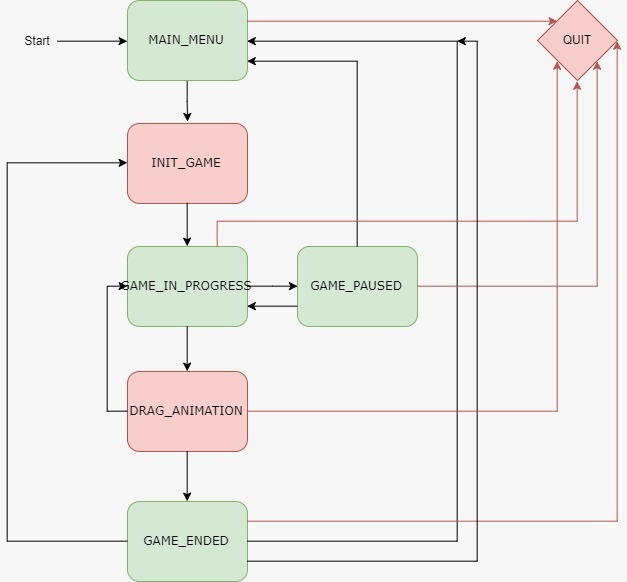
\includegraphics[scale=0.55]{Images/GameStatesBasic.jpeg}
\end{figure}

In the figure below is a more detaild diagram shown on how the states could be implemented in our existing code.
\begin{figure}[H]
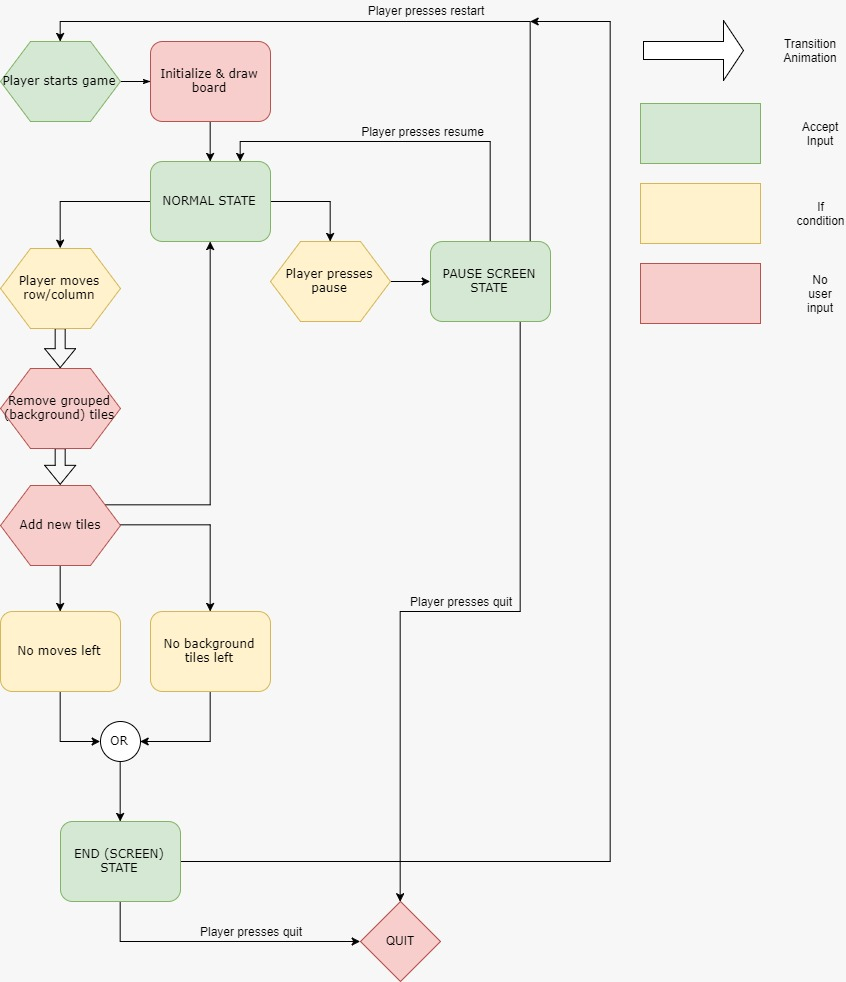
\includegraphics[scale=0.45]{Images/GameStates.jpeg}
\end{figure}


\subsection{Maximum Moves per Level}
Adding a constraint on the amount of moves in each level makes the game more immersive. The player needs to clear all items with a square background around them within a given number of moves. If the player manages to clear all these items within the maximum amount of moves the game will continue until the maximum amount of move are reached. When the player passes the amount of moves the player and the player did not manage to clear all background items the game will end. When the player passes the amount of moves and the player was able to clear all background items, the game will generate a new board and the amount of moves are reset to the default value. 

\subsubsection{Requirements}
The requirement that are sorted using the MoSCoW model.

\paragraph{Must Have}
\begin{itemize}
	\item There must be a maximum amount of moves per level.
	\item The game must end when the maximum amount of moves are reached and not all backgound items are cleared.
	\item The game must continue when the maximum amount of moves are reached and all backgound items are cleared.
	\item When the game continues after the maximum amount of moves are reached the amount of moves left must be reset to the default value.
\end{itemize}
\paragraph{Should Have}
\begin{itemize}
	\item The game should generate a new board when the game continues after the maximum amount of moves are reached.
	\item The default amount of moves should be configurable from the configuration file.
	\item The player should be able to see the amount of moves left.
	\item The score should not be reset once the game continues after the maximum amount of moves are reached.
\end{itemize}


\subsubsection{Software Design}
\begin{tikzpicture}[node distance = 2cm, auto]
    % Place nodes
    \node [block] (nrmoves) {moves left -1};
    \node [cloud, left of=nrmoves] (player) {player move};
	\node [decision, below of=nrmoves] (movesleft) {is moves left 0?};
	\node [decision, below of=movesleft] (item) {background items left?};
	\node [block, below of=item, node distance=3cm] (end) {end game};
	\node [block, left of=item, node distance=3cm] (new) {create new game};
    
    
    \path [line,dashed] (player) -- (nrmoves);
    \path [line] (nrmoves) -- (movesleft);
	\path [line,dashed] (movesleft) -| node {no}(player);   
	\path [line] (movesleft) -- node {yes}(item);
	\path [line] (item) -- node {yes}(end);
	\path [line] (item) -- node {no}(new);    
    
    
    \path [line,dashed] (new) -- (player);
\end{tikzpicture}


\section{Turn-based Multiplayer}
In exercise three we have been asked to implement a feature that we wanted to implement. We have chosen to implement turn-based Multiplayer. For this feature we also created new requirements and a software design.

\subsection{Requirements}
The requirement that are sorted using the MoSCoW model.

\paragraph{Must Have}
\begin{itemize}
	\item There must exists a central server to handle communication between players.
	\item There must be a open port that listening to the player who wants to connect to the network.
	\item A player must be able to connect to a server using an address.
	\item It must be possible to send data to all or some of the player via the server.
	\item When a player move something on the screen all other players must be able to see it live on their screen and sync everything.
	\item There must exists a communication protocol to exchange data between players (via server).
	\item The server must decide who's turn it is to play the game.
	\item When the player connects to the network their game must be put in a pause mode waiting for the server to initiate the game.
	\item The players must be able to see on the screen if they should play the game or wait for other players.
\end{itemize}

\paragraph{Should Have}
\begin{itemize}
	\item The player should see the errors graphically instead of on terminal errors.
	\item A Command design pattern should be implemented to handle the communication protocol.
	\item The server should announce the winner.
\end{itemize}
\paragraph{Could Have}
\begin{itemize}
	\item The player could send their names and see the score of each other on their screen.
\end{itemize}
 

\subsection{Software Design}
\begin{figure}[H]
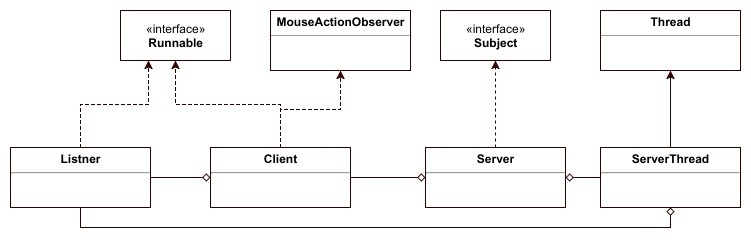
\includegraphics[scale=0.55]{Images/MultiplayerClassDiagram.jpeg}
\end{figure}



\end{document}






